\documentclass{BHCexam}
\biaoti{指数对数}
\fubiaoti{}
\begin{document}
\maketitle
%\tableofcontents
\begin{questions}
\qs 已知$ 0<m<n<1 $,且$ 1<a<b $,则下列各式中一定成立的是\xx
\onech{$ b^m>a^n$}{$ b^m<a^n$}{$ m^b>n^a$}{$ m^b<n^a$}
\qs 已知$ a=2^{\frac{4}{3}} ,b=4^{\frac{2}{5}},c=25^{\frac{1}{3}}$,则\xx
\onech{$ b<a<c$}{$ a<b<c$}{$ b<c<a$}{$ c<a<b$}
\qs 设$ a,b,c $都是正数,且$ 3^a=4^b=6^c $,那么\xx
\onech{$ \dfrac{1}{c}=\dfrac{1}{a}+\dfrac{1}{b}$}{$\dfrac{2}{c}=\dfrac{2}{a}+\dfrac{1}{b} $}{$\dfrac{1}{c}=\dfrac{2}{a}+\dfrac{2}{b} $}{$ \dfrac{2}{c}=\dfrac{1}{a}+\dfrac{2}{b}$}
\qs 设$ \dfrac{1}{2}<\left(\dfrac{1}{2}\right)^b<\left(\dfrac{1}{2}\right)^a<1 $,那么\xx
\onech{$ a^a<a^b<b^a$}{$ a^a<b^a<a^b$}{$ a^b<a^a<b^a$}{$ a^b<b^a<a^a$}
\qs 函数$y=\left(\dfrac{1}{2}\right)^{2x-x^2}$的值域为\xx
\onechx{$ \left[\dfrac{1}{2},+\infty\right)$}{$ \left(-\infty,\dfrac{1}{2}\right]$}{$ \left(0,\dfrac{1}{2}\right]$}{$ \left(0,2\right]$}
\qs 若$ \left(\dfrac{1}{2}\right)^{2a+1} <\left(\dfrac{1}{2}\right)^{3-2a}$,则实数$ a $的取值范围是\xx
\onech{$ \left(-\infty,+\infty\right)$}{$ \left(0,+\infty\right)$}{$ \left(1,+\infty\right)$}{$ \left(0,1\right)$}

\qs 已知函数$f(x)=3^x-\left(\dfrac{1}{3}\right)^x$,则$f(x)$\xx
\twoch{是偶函数,且在$\mathbf{R}$上是增函数}{是奇函数,且在$\mathbf{R}$上是增函数}{是偶函数,且在$\mathbf{R}$上是减函数}{是奇函数,且在$\mathbf{R}$上是减函数}
\qs 已知$ x,y $为正实数,则\xx
\twoch{$ 2^{\lg x+\lg y}=2^{\lg x}+2^{\lg y}$}{$2^{\lg\left( x+ y\right)}=2^{\lg x}\bm{\cdot}2^{\lg y} $}{$ 2^{\lg x\bm{\cdot}\lg y}=2^{\lg x}+2^{\lg y}$}{$ 2^{\lg\left(xy\right)}=2^{\lg x}\bm{\cdot}2^{\lg y}$}
\qs 设$ y_1 =4^{0.9},\ y_2=8^{0.44},\ y_3=\left(\dfrac{1}{2}\right)^{-1.5}$,则\xx
\onech{$ y_3>y_1>y_2$}{$ y_2>y_1>y_3$}{$ y_1>y_2>y_3$}{$ y_1>y_3>y_2$}
\qs 设$ a=\log_32,\ b=\ln2,\ c=5^{-\frac{1}{2}} $,则\xx
\onech{$ a<b<c$}{$ b<c<a$}{$ c<a<b$}{$ c<b<a$}
\qs $ y=0.3^{\abs{x}} $的值域为\xx
\onech{$\left(0,+\infty\right) $}{$ \left[1,+\infty\right)$}{$ \left(-\infty,1\right]$}{$ \left(0,1\right]$}

\qs 设$ 2^a=5^b=m $,且$ \dfrac{1}{a}+\dfrac{1}{b}=2 $,则$ m= $\xx
\onech{$ \sqrt{10}$}{$ 10$}{$ 20$}{$ 100$}
\qs 设$ \log_34\bm{\cdot}\log_48\bm{\cdot}\log_8m=\log_416 $,那么$ m $等于\xx
\onech{$ \dfrac{9}{2}$}{$ 9$}{$ 18$}{$ 27$}
\qs 若$ 0<m<1 $,则\xx
\twoch{$ \log_m{\left(1+m\right)}>\log_m{\left(1-m\right)}$}{$ \log_m{\left(1+m\right)}>0$}{$ 1-m>\left(1+m\right)^2$}{$ \left(1-m\right)^{\frac{1}{3}}>\left(1-m\right)^{\frac{1}{2}}$}

\qs 设$ a=\log_36,b=\log_510,c=\log_714 $,则\xx
\onech{$ c>b>a$}{$ b>c>a$}{$ a>c>b$}{$ a>b>c$}
\qs 设$ a=\lg \mathrm{e} ,b=\left(\lg\mathrm{e}\right)^2,c=\lg\sqrt{\mathrm{e}}$,则\xx
\onech{$ a>b>c$}{$ a>c>b$}{$ c>a>b$}{$ c>b>a$}
\qs 函数$f(x)=2x-2^x$的零点个数是\xx
\onech{$ 1$个}{$2 $个}{$3 $个}{$4 $个}
\qs 若$ 0<a<1,b<-1 $,则$f(x)=a^x+b$的图像不经过\xx
\onech{第一象限}{第二象限}{第三象限}{第四象限}
\qs 已知$f(x)=a^x\ (a>1),g(x)=b^x\ (b>1)$当$ f(x_1)=g(x_2)=2 $时,有$ x_1>x_2 $,则$ a,\ b $的大小关系是\xx
\onech{$ a=b$}{$ a>b$}{$ a<b$}{不能确定}
\qs 若函数$y=a^x+b-1(a>0\text{且}a\ne1)$的图象经过第二、三、四象限,则一定有\xx
\onech{$ 0<a<1\text{且}b>0$}{$ a>1\text{且}b>0$}{$0<a<1\text{且}b<0 $}{$a>1\text{且}b<0 $}


\qs 函数$f(x)=a^{\abs{x+1}}(a>0\text{且}a\ne1)$的值域为$ \left[1,+\infty\right) $,则$ f(-4) $与$ f(1) $的大小关系是\xx
\onech{$ f(-4)>f(1)$}{$ f(-4)=f(1)$}{$ f(-4)<f(1)$}{不能确定}


\qs 已知定义在$ \mathbf{R} $上的奇函数$f(x)$和偶函数$g(x)$满足$ f(x)+g(x)=a^x-a^{-x}+2\ (a>0\text{且}a\ne 1) $.若$ g(2)=a $,则$ f(2)= $\xx
\onech{$2 $}{$ \dfrac{15}{4}$}{$ \dfrac{17}{4}$}{$ a^2$}

\qs 已知函数$ y=a^x,~y=x^b,~y=\log_cx $的图象如图所示,则\xx
\begin{center}
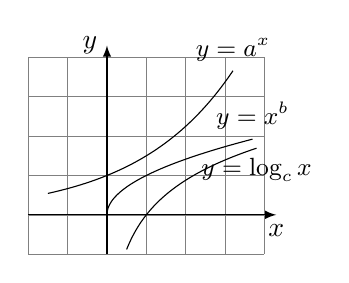
\begin{tikzpicture}[scale=0.5]
\draw[help lines] (-2,-1) grid (4,4);
\draw[->,>=latex](-2,0)--(4.3,0) node[below]{$x$};
\draw[->,>=latex](0,-1)--(0,4.3)node[left]{$y$};
\draw[domain=-1.5:3.2,samples=1000] plot(\x,{(1.5)^\x}) node[above] {\small $y = a^x$};
\draw[domain=0:3.7,samples=1000] plot(\x,{\x^0.5})node[above] {\small $y = x^b$};
\draw[domain=0.5:3.8,samples=1000] plot(\x,{log2(\x)/log2(2.2})node[below]{\small $y=\log_cx$};
\end{tikzpicture}
\end{center}
\vspace{-1em}
\onech{$ a>b>c$}{$ a>c>b$}{$ c>a>b$}{$ c>b>a$}
\qs 函数$f(x)=\dfrac{1}{2^x+1}$在$ \left(-\infty,+\infty\right) $上\xx
\twoch{单调递减无最小值}{单调递减有最小值}{单调递增无最大值}{单调递增有最大值}
\qs 根据有关资料,围棋状态空间复杂度的上限$ M $约为$ 3^{361} $,而可观测宇宙中可观测物质的总数$ N $约为$ 10^{80} $.则下列各数中与$ \dfrac{M}{N} $最接近的是\xx\\
(参考数据:$ \lg 3\approx 0.48 $)\\
\onech{$ 10^{33}$}{$ 10^{53}$}{$ 10^{73}$}{$ 10^{93}$}
\qs 如图,点$A,~B$在函数$ y=\log_2x+2 $的图象上,点$C$在函数$y=\log_2x$的图象上,若$ \triangle ABC$为等边三角形,且直线$ BC\sslash y$轴,设点$A$的坐标为$ (m,n) $,则$ m= $\xx
\vspace{-1em}
\begin{center}
	\begin{tikzpicture}[domain=0.1:4,scale=0.6]
	\clip (-0.5,-1) rectangle (5,5);
	\tikzmath{
		\i=sqrt(3);
		\a=log2(\i);
		\b=\i+sqrt(3);
		\c=log2(\b);
		\d=\c+2;
	}
	%    \draw[very thin,color=gray] (0.1,-1.1) grid (3.9,3.9);
	\draw[->] (-0.2,0) -- (4.2,0) node[right] {$x$};
	\draw[->] (0,-1.2) -- (0,4.2) node[above] {\small$f(x)$};
	\draw plot(\x,{log2(\x)+2});%node[above]{$f(x)=log_2x+2$}; 
	\draw plot(\x,{log2(\x)});%node[above]{$f(x)=log_2x$}; 
	\coordinate [label=left:\small$A$] (A) at($(\i,\a+2)$);
	\coordinate [label=above:\small$B$] (B) at($(\b,\d)$);
	\coordinate [label=below:\small$C$] (C) at($(\b,\c)$);
	\draw(A)--(B)--(C)--cycle;
	\end{tikzpicture}
\end{center}
\vspace{-2em}
\onech{$2$}{$3$}{$ \sqrt{2} $}{$ \sqrt{3} $}
\qs 如图所示,$A$是函数$ f(x)=2^x $的图象上的动点,过点$ A $作直线平行于$ x $轴,交函数$ g(x)=2^{x+2} $的图象于点$ B $,若函数$f(x)=2^x$的图象上存在点$ C $使得$ \triangle ABC $为等边三角形,则称$ A $为函数$ f(x)=2^x $上的好位置点.函数$ f(x)=2^x $上的好位置点的个数为\xx
\begin{center}
\begin{tikzpicture}[scale=0.3]

\tikzmath{
\a=sqrt(5);
}
\draw[->,>=latex](-2,0)--(3,0) node[below]{$x$};
\draw[->,>=latex](0,-2)--(0,8) node[right]{$y$};
\node[below left] (O) at(0,0) {$O$};
%\clip (-2,-2) rectangle (4,7);
\draw[domain=-1.5:3,samples=1000] plot(\x,{2^\x});
\draw[domain=-1.5:1,samples=1000] plot(\x,{2^(\x+2)});
\draw (-1,5)--(3,5);
%\node[above right] (A) at(\a,5) {\small $A$};
%\node[above right] (B) at(\a-2,5) {\small $B$};
\draw[fill=black](\a+0.07,5)circle(2 pt) node[above right]  {\small $A$};

\draw[fill=black](\a-2+0.07,5) circle(2 pt) node[above right]  {\small $B$};;

\end{tikzpicture}
\end{center}
\vspace{-2em}
\onech{$ 0$}{$ 1$}{$ 2$}{$ 3$}

\qs 已知函数$f(x)=\begin{dcases}
2^x,&x\le0,\\
\sqrt{x},&x>0.
\end{dcases}$若函数$g(x)=f(x)-k(x-1)$有且只有一个零点,则实数$ k $的取值范围是\xx
\onech{$\left(-\infty,1\right) $}{$ \left(0,+\infty\right)$}{$ \left(-1,0\right)$}{$ \left(-\infty,-1\right)\bigcup\left(0,\infty\right)$}
\qs 不等式$ 2^{x^2-x}<4 $的解集为\tk.
\qs 计算:$\lg 25+\lg2\times \lg 50+\left(\lg2\right)^2$=\tk.
\qs 若$ \ln a>0,\log_32^b<-1,c^2\le1, $那么$ a,b,c $中最大的一个是\tk.
\qs 已知$ \left(a^2+2a+5\right)^{3x}>\left(a^2+2a+5\right)^{1-x} $,则$x$的取值范围是\tk.
\qs 已知函数$f(x)=\begin{dcases}
2^x+a,&x\ge0,\\
x^2-ax,&x<0.
\end{dcases}$若$f(x)$的最小值是$ a $,则$ a =$\tk.
\qs 已知函数$f(x)=a^x+b\left(a>0,a\ne1\right)$的定义域和值域都是$[-1,0]$,则$ a+b =$\tk.
\end{questions}
\end{document}